\chapter{Implementierung}
\label{ch:implementation}

In diesem Kapitel wird die Implementierung der Anwendung beschrieben.
Hierbei wird exemplarisch auf zwei wichtige Funktionen der Anwendung eingegangen.
Diese sind die Verwaltung des Benutzerprofils und die Erstellung und Anzeige von Beiträgen.

Da der komplette Code und viele Screenshots den Rahmen dieses Kapitels sprengen würden, wird in den einzelnen Kapiteln nur ein Auszug gezeigt.
Den kompletten Code findet man direkt im Github Repository unter \url{https://github.com/Jonasdero/digital-hometown-frontend}.

\section{Profil}
\label{sec:profile}

Die Profile eines Nutzers sind in der Anwendung sehr wichtig.
Jeder Nutzer verwaltet sein eigenes Profil, welches er mit anderen Nutzern teilt.
Dazu gehören Informationen wie Name, E-Mail-Adresse, Geburtsdatum, Geschlecht und ein Profilbild.
Damit andere Nutzer die Informationen des Profils sehen können, muss das Profil öffentlich sein.
Zudem sollen Benutzer der Anwendung durch Interessen, Profilbilder und persönliche Beschreibungen voneinander unterscheidbar sein und sich so besser vernetzen können.
Um sich mit anderen Nutzern zu verbinden, ist es wichtig, dass diese Informationen in der Anwendung gespeichert werden.

Außerdem soll die soziale Interaktion zwischen Nutzer ermöglicht werden.
Dazu gehören Funktionen wie das Folgen von anderen Nutzern oder auch das Schreiben von Nachrichten zwischen zwei Nutzern oder in Gruppen.
Dies soll direkt vom Profil eines Nutzers aus möglich sein.

\begin{figure}[ht!]
  \begin{centering}
    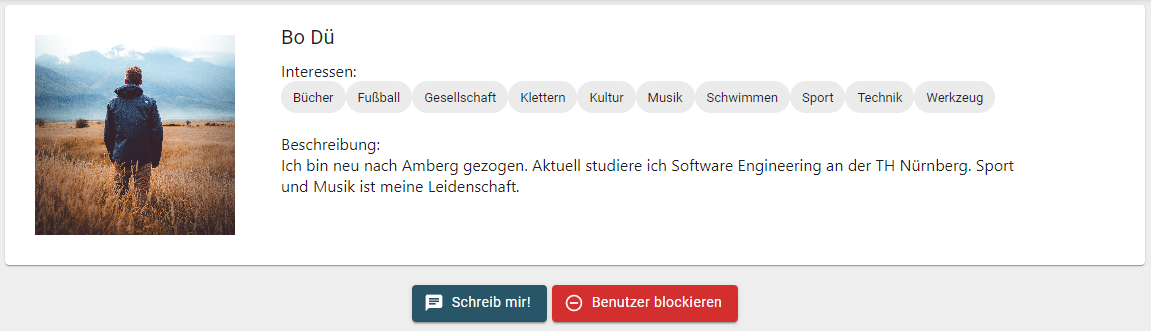
\includegraphics[width=1\textwidth]{figures/implementation/profile-header.png}
    \caption{Übersicht eines Benutzerprofils}
    \label{fig:userProfileHeader}
  \end{centering}
\end{figure}

Hier sieht man die verschiedenen Informationen, die ein Nutzer in seinem Profil angeben kann.
In den nächsten Seiten wird die Implementierung dieser Funktionen beschrieben.
Diese wird aufgeteilt in die verschiedenen Bereiche: \textit{Anmeldung \& Registrierung}, \textit{persönliches Accountmanagement}, \textit{Profilseite \& Profilbilder} und \textit{blockierte Nutzer}.

\subsection{Anmeldung \& Registrierung}
\label{sec:login}

Den Nutzern wird die Möglichkeit gegeben, sich mit einer E-Mail-Adresse und einem Passwort anzumelden oder eine direkte Anmeldung über OAuth mit Google zu nutzen.
Dies wird beides durch die Firebase Authentication API ermöglicht.

Sobald ein Nutzer sich registriert hat, wird von Firebase intern ein Benutzerprofil erstellt, welches wichtige Nutzermetadaten und Authentifizierungsinformationen enthält.
Außerdem wird bei der Anmeldung über Google das Profilbild mit in Firebase gespeichert.
Die Anmeldemaske sieht wie folgt aus:

\begin{figure}[ht!]
  \begin{centering}
    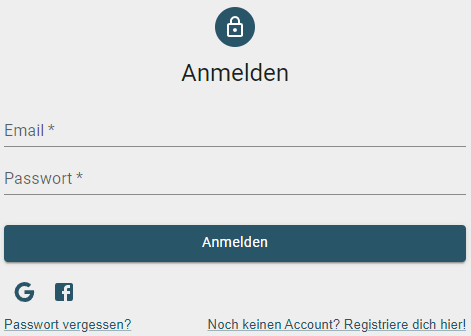
\includegraphics[width=.75\textwidth]{figures/implementation/anmeldemaske.png}
    \caption{Anmeldemaske}
    \label{fig:login}
  \end{centering}
\end{figure}

Um diese Daten in der Anwendung zu speichern, wird ein eigener Benutzerdatensatz angelegt, sobald ein Nutzer registriert wurde und Daten aus dem internen Benutzerprofil von Firebase mit übertragen.
Hierbei wird unterschieden, ob der aktuelle Benutzer ein normaler Nutzer oder ein Verein ist.
Diese werden in unterschiedlichen „Collections“ gespeichert.
Bei der Anmeldung wird dann geprüft, welchen Typ der Benutzer hat und die Daten entsprechend geladen.
Dadurch kann mit einer Datenstruktur gearbeitet werden, die für beide Typen geeignet ist.
Andere Ansichten basieren dann häufig auf der Unterscheidung zwischen Nutzern und Vereinen.
Die Struktur des Datensatzes kann man in Abbildung \ref{fig:firestoreUser} sehen.

\clearpage

\subsection{Persönliches Accountmanagement}
\label{sec:accountmanagement}

Um die Daten des Benutzerprofils zu verwalten, gibt es eine Seite, auf der der Nutzer seine persönlichen Daten ändern kann.
Diese werden dann in der Anwendung aktualisiert und in der Datenbank gespeichert. Er hat hier die Möglichkeit seinen Namen, seine E-Mail, sein Geburtsdatum und seine Postleitzahl zu ändern.
Hier kann außerdem der komplette Account gelöscht werden, um die Daten des Nutzers zu löschen.

\begin{figure}[ht!]
  \begin{centering}
    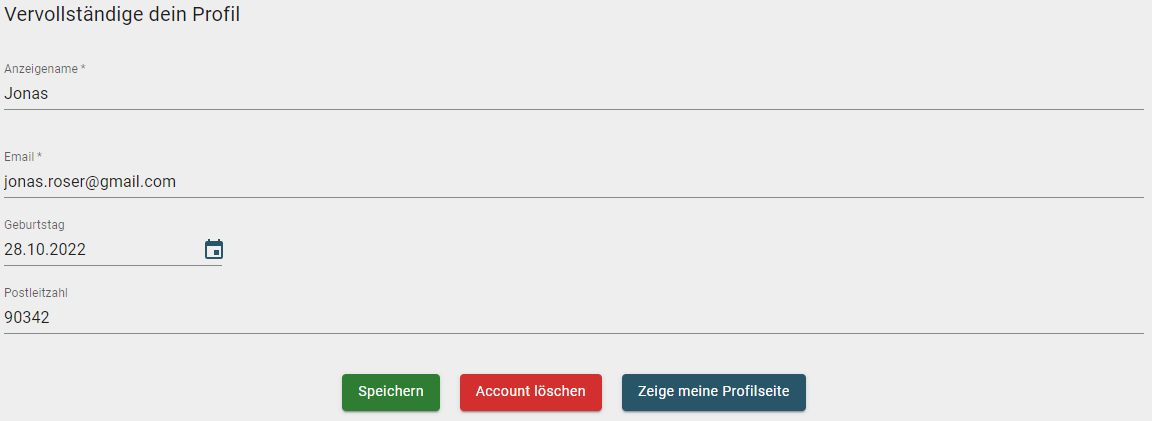
\includegraphics[width=1\textwidth]{figures/implementation/userSettings.png}
    \caption{Benutzereinstellungen}
    \label{fig:userSettings}
  \end{centering}
\end{figure}

\subsection{Profilseite \& Profilbilder}
\label{sec:profilepictures}

Auf der Profilseite des Nutzers kann er seine persönlichen Daten einsehen und bearbeiten. Hier können Interessen und eine Beschreibung hinzugefügt werden.
Außerdem kann er sein Profilbild ändern, indem er auf das Profilbild oder auf den Knopf mit der Kamera klickt.
Dies wird dann im Firebase Storage gespeichert und in der Datenbank verlinkt.

Das Ganze ist so aufgebaut, dass Nutzer zwischen einer Vorschau, also der Sicht, die auch andere Nutzer von seinem Profil sehen und der Bearbeitungssicht unterscheiden können.

\begin{figure}[ht!]
  \begin{centering}
    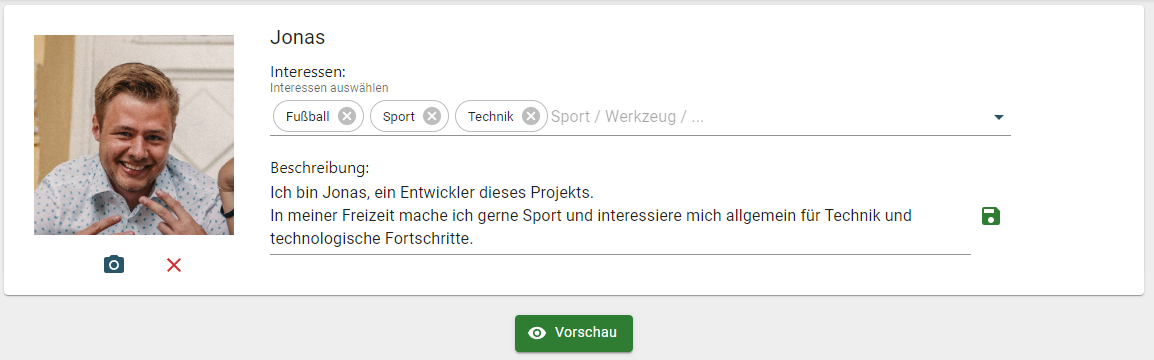
\includegraphics[width=1\textwidth]{figures/implementation/my-profile-header.png}
    \caption{Persönliches Profil}
    \label{fig:myProfileHeader}
  \end{centering}
\end{figure}

\subsection{Blockierte Nutzer}
\label{sec:blockedusers}

Um die Privatsphäre der Nutzer zu schützen, können diese andere Nutzer blockieren.
Blockierte Nutzer können dann nicht mehr auf das Profil des Blockierenden zugreifen und auch keine Nachrichten mehr schreiben.

Über die Profilseite kann ein Nutzer einen anderen Nutzer blockieren.

\begin{figure}[ht!]
  \begin{centering}
    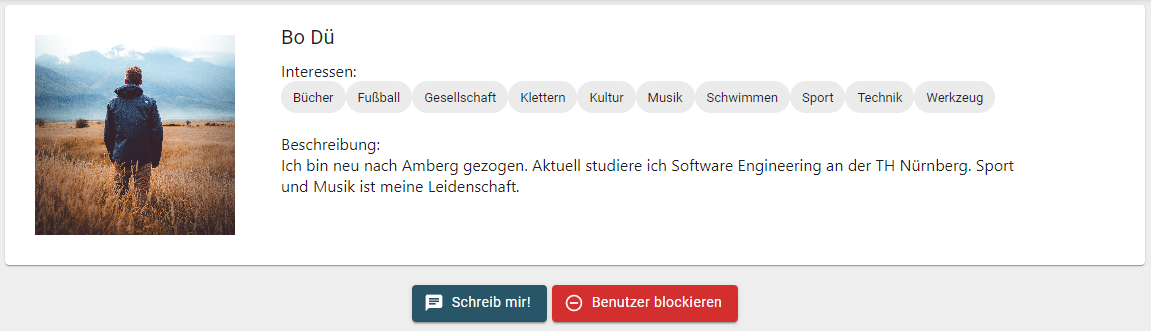
\includegraphics[width=1\textwidth]{figures/implementation/profile-header.png}
    \caption{Blockieren eines Nutzers}
    \label{fig:blockUser}
  \end{centering}
\end{figure}

Blockierte Nutzer kann man dann in der Anwendung unter dem Menüpunkt \textit{Blockiert} einsehen.
Dort wird jeder Nutzer oder Verein aufgeführt, welcher blockiert ist.
Mit einem Klick auf das „X“ wird der Block aufgehoben.

\begin{figure}[ht!]
  \begin{centering}
    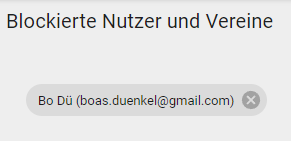
\includegraphics[width=.5\textwidth]{figures/implementation/blocked.png}
    \caption{Blockierte Nutzer}
    \label{fig:blocked}
  \end{centering}
\end{figure}

\section{Beiträge}
\label{sec:contributions}

Beiträge sind ein anderes wichtiges Feature von „Digital Dahoam“.
Hiermit können Nutzer Informationen austauschen, die für andere Nutzer interessant sein könnten.
Beiträge können von allen Nutzern erstellt werden, die sich registriert haben.
Es gibt folgende Typen von Beiträgen:

\begin{itemize}
  \item \textbf{Anfrage}: Hier können Nutzer eine Anfrage stellen, die dann von anderen Nutzern beantwortet werden kann. Anfragen können auch benutzt werden, wenn bestimmte Gegenstände im Haushalt fehlen, z. B. ein bestimmtes Werkzeug oder ein bestimmtes Lebensmittel.
  \item \textbf{Angebot}: Hier können Nutzer ein Angebot erstellen, das dann von anderen Nutzern angenommen werden kann. Dies kann wie Ebay-Kleinanzeigen benutzt werden, um überflüssige Gegenstände zu verkaufen.
  \item \textbf{Information}: Hier können Nutzer Informationen teilen, die für andere Nutzer interessant sein könnten.
  \item \textbf{Veranstaltung}: Hier können Nutzer Veranstaltungen erstellen, die dann von anderen Nutzern besucht werden können.
\end{itemize}

\subsection{Beiträge erstellen}
\label{sec:createpost}

Beiträge können mit einem Klick auf den Button \textit{Beiträge erstellen} erstellt werden.
Hier öffnet sich ein Pop-up, welchem der Nutzer den Titel, die Beschreibung, den Beitragstyp und die Kategorie des Beitrags eingeben kann.
Außerdem werden für jeden Beitrag das Startdatum, also ab wann der Beitrag gültig ist und angezeigt wird, und das Enddatum, also bis wann der Beitrag gültig ist und angezeigt wird, festgelegt.
Für Veranstaltungen gibt es zusätzlich noch den Ort und das Datum.
Sobald auf \textit{absenden} geklickt wird, wird der Beitrag in der Datenbank gespeichert und auf der Startseite angezeigt.

\begin{figure}[ht!]
  \begin{centering}
    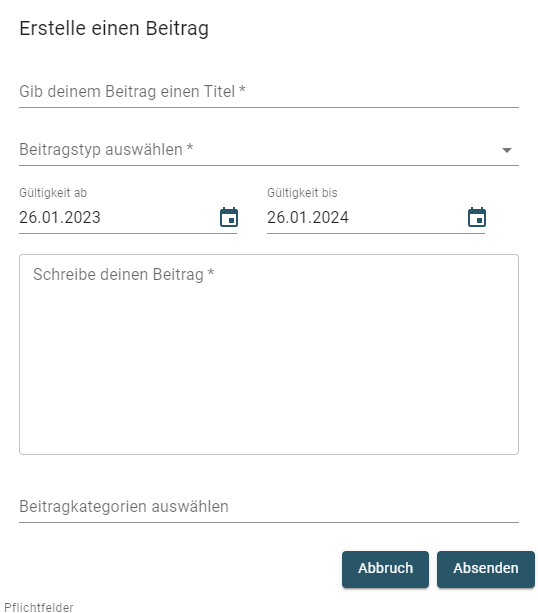
\includegraphics[width=.65\textwidth]{figures/implementation/createpost.png}
    \caption{Beiträge erstellen}
    \label{fig:createpost}
  \end{centering}
\end{figure}


\subsection{Alle Beiträge}
\label{sec:allposts}

Unter \textit{Alle Beiträge} findet man alle Beiträge, die ein valides Gültigkeitsdatum haben. Diese werden mit Titel, Beschreibung, Kategorie und Beitragstyp angezeigt.
Für Veranstaltungen gibt es zusätzlich noch den Ort und das Datum.

\begin{figure}[ht!]
  \begin{centering}
    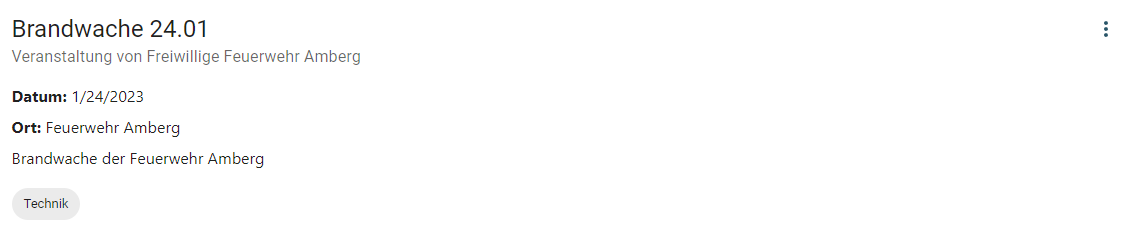
\includegraphics[width=.8\textwidth]{figures/implementation/beitrag.png}
    \caption{Beitrag}
    \label{fig:beitrag}
  \end{centering}
\end{figure}

Ein Problem, was es während der Implementierung zu lösen galt, war die richtige Filterung der Beiträge. Die hier verwendete Sortierfunktion (siehe \ref{code:filterPosts}) wurde dann für die restlichen Listen verwendet und die gefilterten Beiträge dort nur noch verfeinert.
Diese musste folgendes erfüllen:

\begin{itemize}
  \item Eigene Beiträge werden immer angezeigt.
  \item Beiträge, die nicht mehr gültig sind, werden nicht angezeigt.
  \item Beiträge von blockierten Nutzern werden nicht angezeigt.
  \item Beiträge müssen nach Datum sortiert werden.
\end{itemize}

Mit dem Klick auf die 3 kleinen Punkte in der rechten oberen Ecke öffnet man das Beitragsmenü. Hier gibt es folgende Punkte:

\begin{itemize}
  \item \textbf{Beitrag zum Merkzettel}: Hinzufügen eines Inhalts zum Merkzettel.
  \item \textbf{Details}: Anzeigen der Details des Beitrags. (siehe \ref{fig:details})
  \item \textbf{Zum Autor}: Direkter Link zum Profil des Autors.
  \item \textbf{Nachricht an Autor}: Direkter Link zur Nachrichtenfunktion, um dem Autor eine Nachricht zu schicken.
\end{itemize}

\begin{figure}[ht!]
  \begin{centering}
    \includegraphics[width=.25\textwidth]{figures/implementation/beitragsmenü.png}
    \caption{Beitragsmenü}
    \label{fig:beitragsmenü}
  \end{centering}
\end{figure}

\clearpage
\subsection{Profilseite}
\label{sec:profilepage}

Auf der Profilseite kann der Nutzer werden seine Beiträge angezeigt.
Hier werden auch abgelaufene Beiträge angezeigt und grau hinterlegt.

\begin{figure}[ht!]
  \begin{centering}
    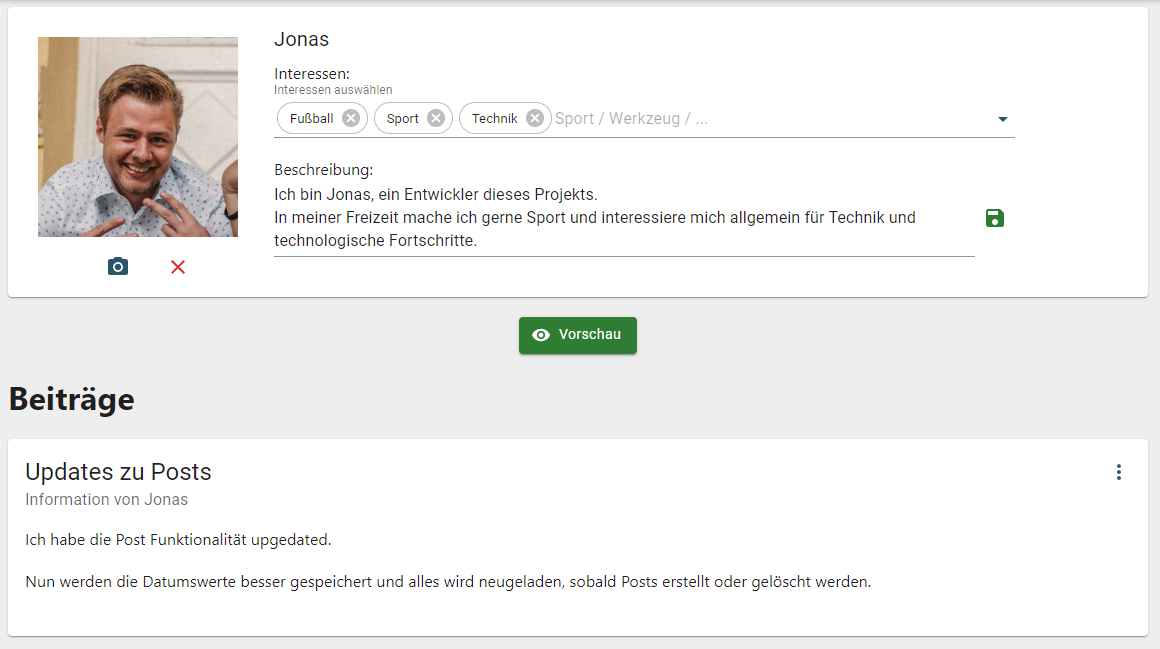
\includegraphics[width=1\textwidth]{figures/implementation/userposts.png}
    \caption{Beiträge des Nutzers}
    \label{fig:userposts}
  \end{centering}
\end{figure}

\subsection{Merkzettel}
\label{sec:bookmark}

Beiträge, die für den Merkzettel markiert sind erscheinen dort, und können dort auch wieder entfernt werden.
Außerdem werden sie nach Beitragstyp gruppiert.

\begin{figure}[ht!]
  \begin{centering}
    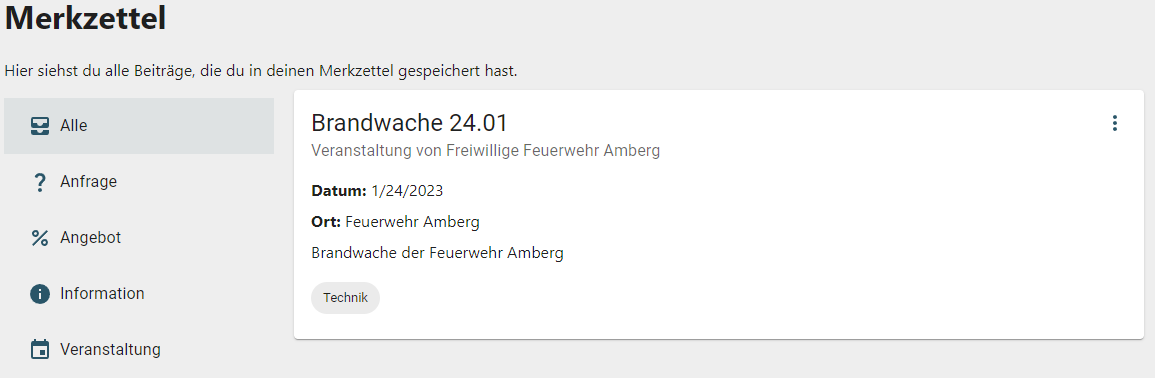
\includegraphics[width=1\textwidth]{figures/implementation/merkzettel.png}
    \caption{Merkzettel}
    \label{fig:merkzettel}
  \end{centering}
\end{figure}

\clearpage
\subsection{Marktplatz}
\label{sec:marketplace}

Auf dem Marktplatz können Personen und Beiträge durchsucht werden.
Durch den Filter auf Kategorien, Informationen oder Veranstaltungen findet man schnell den richtigen Beitrag.

\begin{figure}[ht!]
  \begin{centering}
    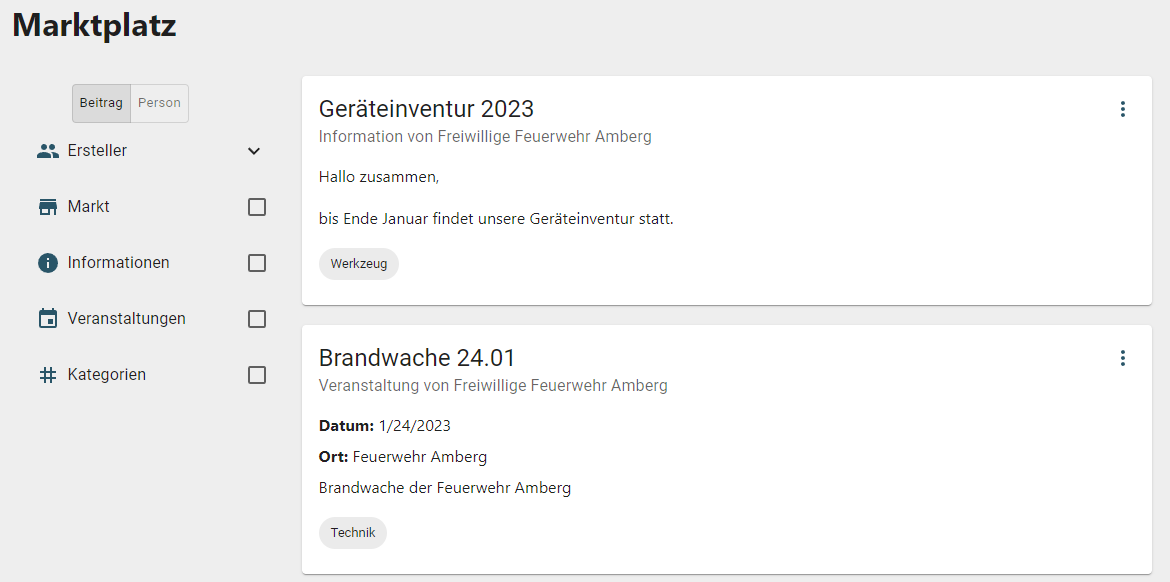
\includegraphics[width=1\textwidth]{figures/implementation/marktplatz.png}
    \caption{Marktplatz}
    \label{fig:marktplatz}
  \end{centering}
\end{figure}


\subsection{Dashboard}
\label{sec:dashboard}

Auf der Startseite werden aktuelle Beiträge aus der Nähe angezeigt, sowie die Veranstaltungen, die der Nutzer auf dem Merkzettel hat.

\begin{figure}[ht!]
  \begin{centering}
    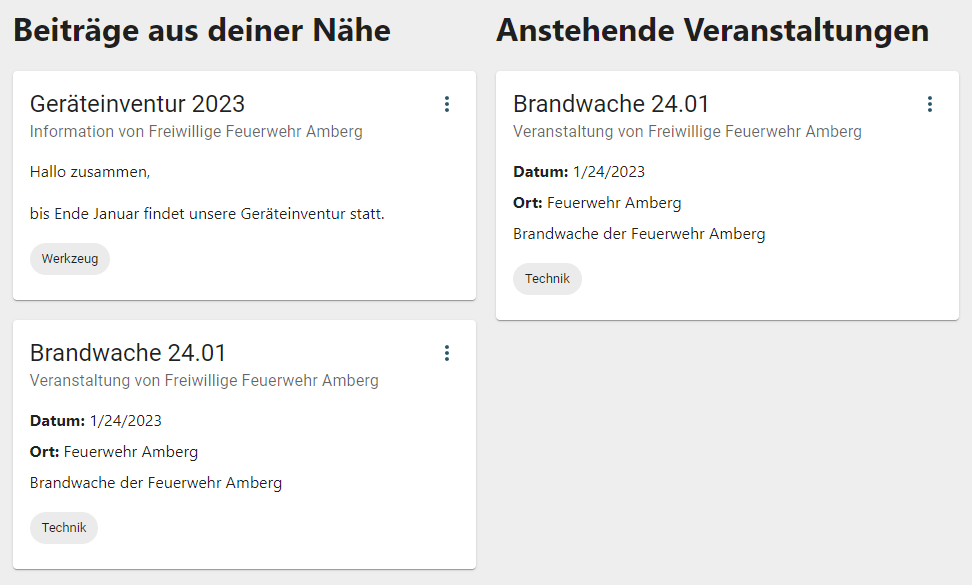
\includegraphics[width=.8\textwidth]{figures/implementation/dashboard.png}
    \caption{Dashboard}
    \label{fig:dashboard}
  \end{centering}
\end{figure}
